%!TEX root = ../main.tex
\section{Data}
\subsection{Factor return series}
Factor return series are downloaded from Ken French's data library.\footnote{\url{http://mba.tuck.dartmouth.edu/pages/faculty/ken.french/data_library.html}} We download the daily momentum factor data set and merge this with the Fama-French 5 factor data set. Both are available since 1963-07-01, making 1963-07-05 the first week of data. We convert each of the return series into weekly log returns for further use. 

[EXPLAIN THE FACTORS]

[DISCUSS ROOT OF THE DATA, CRSP ETC]

% Table created by stargazer v.5.2 by Marek Hlavac, Harvard University. E-mail: hlavac at fas.harvard.edu
% Date and time: lör, okt 15, 2016 - 22:22:53
\begin{table}[!htbp] \centering 
\begin{tabularx}{\textwidth}{X}
  \\[-1.8ex]\toprule
  \\[-1.8ex] 
  \footnotesize Summary statistics of weekly log returns on factor strategies. Kurtosis is excess kurtosis, standardized to zero. 
\end{tabularx}
  \caption{Summary statistics of data} 
  \label{tab:summarydata} 
\begin{tabular}{@{\extracolsep{5pt}} ccccccc} 
\\[-1.8ex]\hline 
\hline \\[-1.8ex] 
 & Mkt.RF & HML & SMB & Mom & RMW & CMA \\ 
\hline \\[-1.8ex] 
nobs & $2,766$ & $2,766$ & $2,766$ & $2,766$ & $2,766$ & $2,766$ \\ 
Maximum & $0.126$ & $0.117$ & $0.060$ & $0.120$ & $0.094$ & $0.054$ \\ 
Minimum & $$-$0.198$ & $$-$0.083$ & $$-$0.098$ & $$-$0.175$ & $$-$0.062$ & $$-$0.044$ \\ 
Mean & $0.001$ & $0.001$ & $0.0003$ & $0.001$ & $0.001$ & $0.001$ \\ 
Median & $0.003$ & $0.0005$ & $0.001$ & $0.002$ & $0.0005$ & $0.0004$ \\ 
Standard deviation & $0.022$ & $0.012$ & $0.012$ & $0.019$ & $0.009$ & $0.009$ \\ 
Skewness & $$-$0.688$ & $0.331$ & $$-$0.504$ & $$-$1.390$ & $0.724$ & $0.306$ \\ 
Excess kurtosis & $6.191$ & $7.318$ & $4.997$ & $11.987$ & $13.005$ & $3.149$ \\ 
\hline \\[-1.8ex] 
\end{tabular} 
\end{table}

[BRIEFLY DISCUSS SUMMARY STATS]

\begin{figure}[H]
  \caption{Cumulative returns to factor strategies}
  \label{diag:cumret}
  \toprule
  \centering
  \begin{minipage}{\textwidth}
  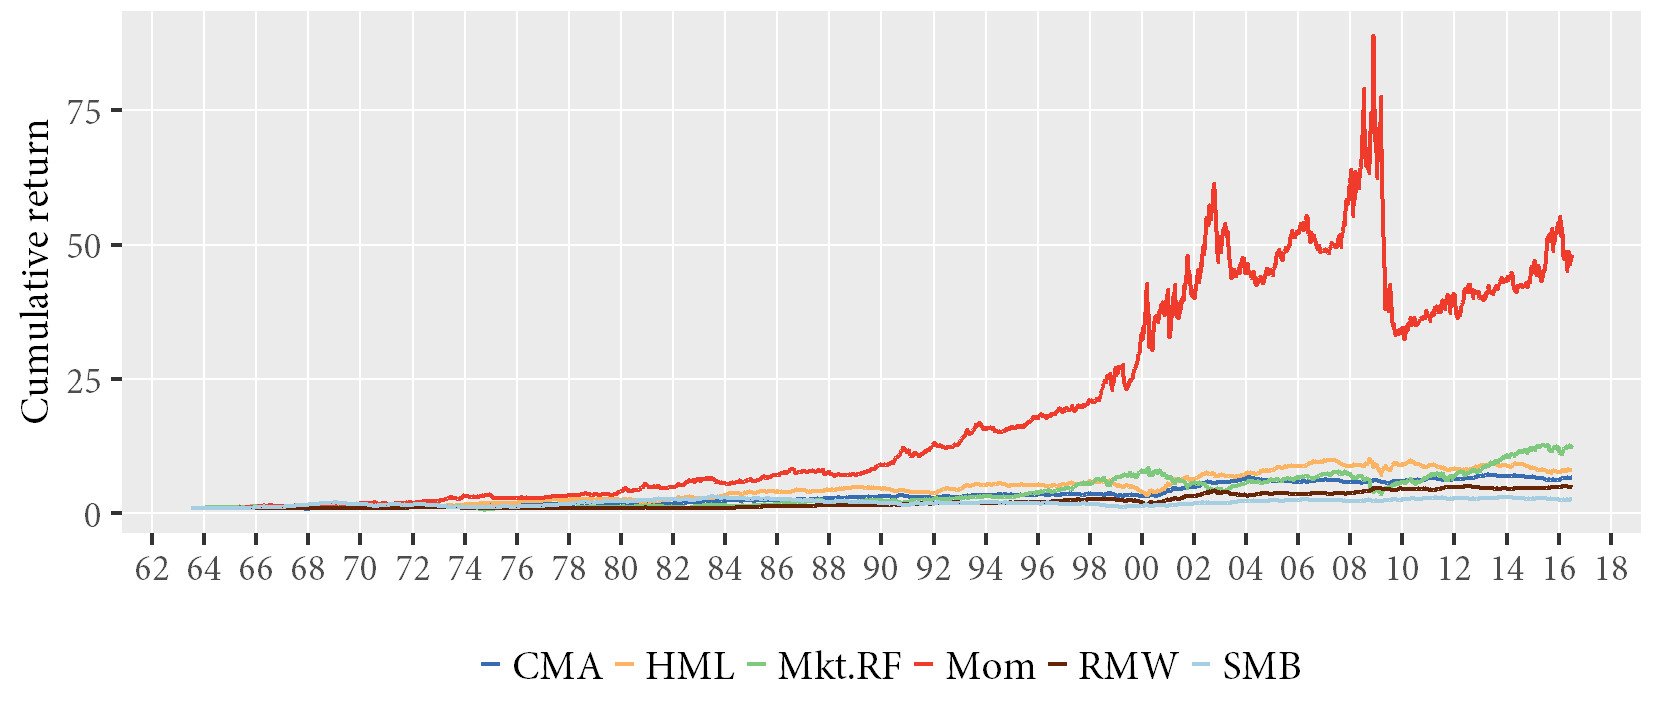
\includegraphics[scale=1]{graphics/cumretPlot.png}  
  \bottomrule
  \vspace{3mm}
  \footnotesize
  Cumulative returns to investing one dollar in each factor strategy beginning 1963-07-05.  All data 1963-07-05 - 2016-07-01.
  \end{minipage}
\end{figure}

\begin{figure}[H]
  \caption{Standardized cumulative returns to factor strategies}
  \label{diag:cumretstd}
  \toprule
  \centering
  \begin{minipage}{\textwidth}
  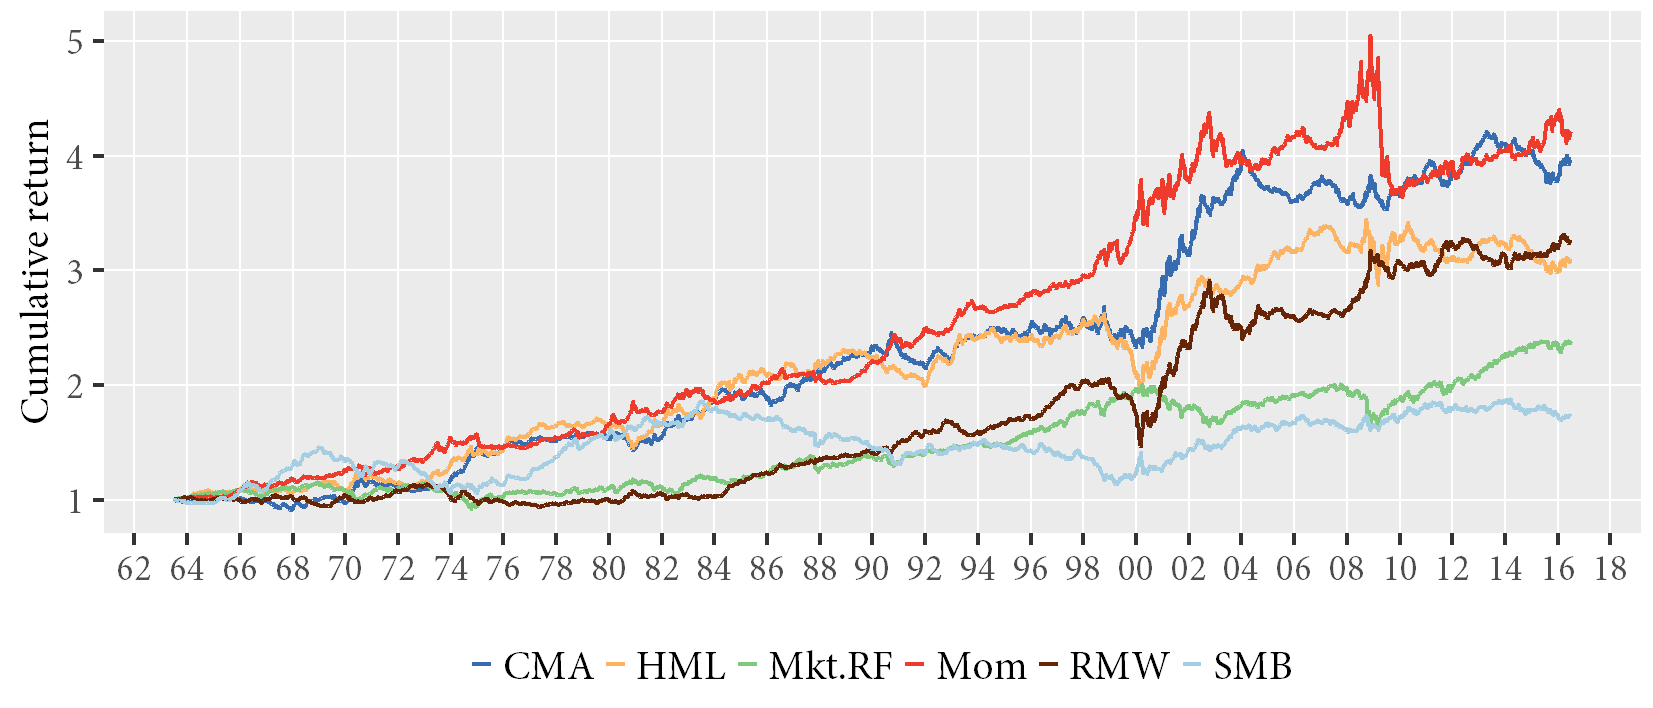
\includegraphics[scale=1]{graphics/cumretStdPlot.png}  
  \bottomrule
  \vspace{3mm}
  \footnotesize
  Cumulative returns to investing one dollar in each factor strategy beginning 1963-07-05. Standardized to 10\% annual volatility. All data 1963-07-05 - 2016-07-01.
  \end{minipage}
\end{figure}

[BRIEFLY DISCUSS FIGURE]